This section provides a detailed explanation of the data collection, graph construction, and embedding extraction processes, as well as the methodology that leverages Graph Neural Networks (GNNs) to compute high-dimensional embeddings.
\subsection{Graph Convolution using Chebyshev Polynomials}
Let \( G = (V, E) \) be an undirected graph with adjacency matrix \( A \) and degree matrix \( D \). The normalized Laplacian matrix is defined as:
\begin{equation}
	\mathcal{L} = I - D^{-1/2} A D^{-1/2}
\end{equation}

Chebyshev graph convolutions approximate spectral filtering using Chebyshev polynomials:
\begin{equation}
	X^{(l+1)} = \sum_{i=0}^{k} \theta_i T_i(\tilde{\mathcal{L}}) X^{(l)}
\end{equation}

where:
\begin{itemize}
	\item $X^{(l)}$ is the feature matrix at layer $l$,
	\item $T_i(\tilde{\mathcal{L}})$ are Chebyshev polynomials of the normalized Laplacian $\tilde{L}$,
	\item $\theta_i$ are trainable coefficients,
	\item $k$ is the Chebyshev polynomial order.
\end{itemize}



\subsection{Adaptive Receptive Fields}
We introduce an adaptive mechanism where the polynomial order \( k \) is dynamically adjusted based on node importance:
\begin{equation}
	k_v = \min(k_{max}, \alpha \cdot \log(\deg(v) + 1))
\end{equation}
where \( \deg(v) \) is the degree of node \( v \), and \( \alpha \) is a tunable scaling factor.


\subsection{Optimization and Training}

To enhance computational efficiency, ACGNN incorporates several optimizations within its adaptive Chebyshev network. The Chebyshev order is reduced from $k=3$ to $k=2$, minimizing computational overhead while maintaining performance. Instead of LayerNorm, BatchNorm is employed to accelerate training. The architecture is further streamlined by reducing the number of ChebConv layers from three to two, lowering model complexity. Additionally, residual connections are introduced after the first layer, facilitating more efficient gradient flow and improving convergence speed. These modifications collectively enhance ACGNN’s efficiency without compromising its predictive capabilities.
Let $|E|$ be the number of edges and $F$ the feature dimension, the computational complexity of ACGNN  compared to standard ChebNet are shown in Table~\ref{tab:comp_cost}.
\begin{table}[h]
	\centering
	\captionsetup{font=small}
\scriptsize
	\begin{tabular}{lccc}
		\toprule
		Model & ChebConv Layers & Normalization & Complexity ($O(\cdot)$) \\
		\midrule
		Standard ChebNet & 3 & LayerNorm & $3k |E| F^2$ \\
		Adaptive ChebNet & 2 & BatchNorm & \textbf{$2k |E| F^2$} \\
		\bottomrule
	\end{tabular}
	\caption{Comparison of Computational Cost}
	\label{tab:comp_cost}
\end{table}



%\vspace{0.5cm} % 
\begin{figure*}
	\centering
	\scriptsize
	%\captionsetup{font=scriptsize}
	\captionsetup{font=footnotesize}
	%%\captionsetup{font=scriptsize}
	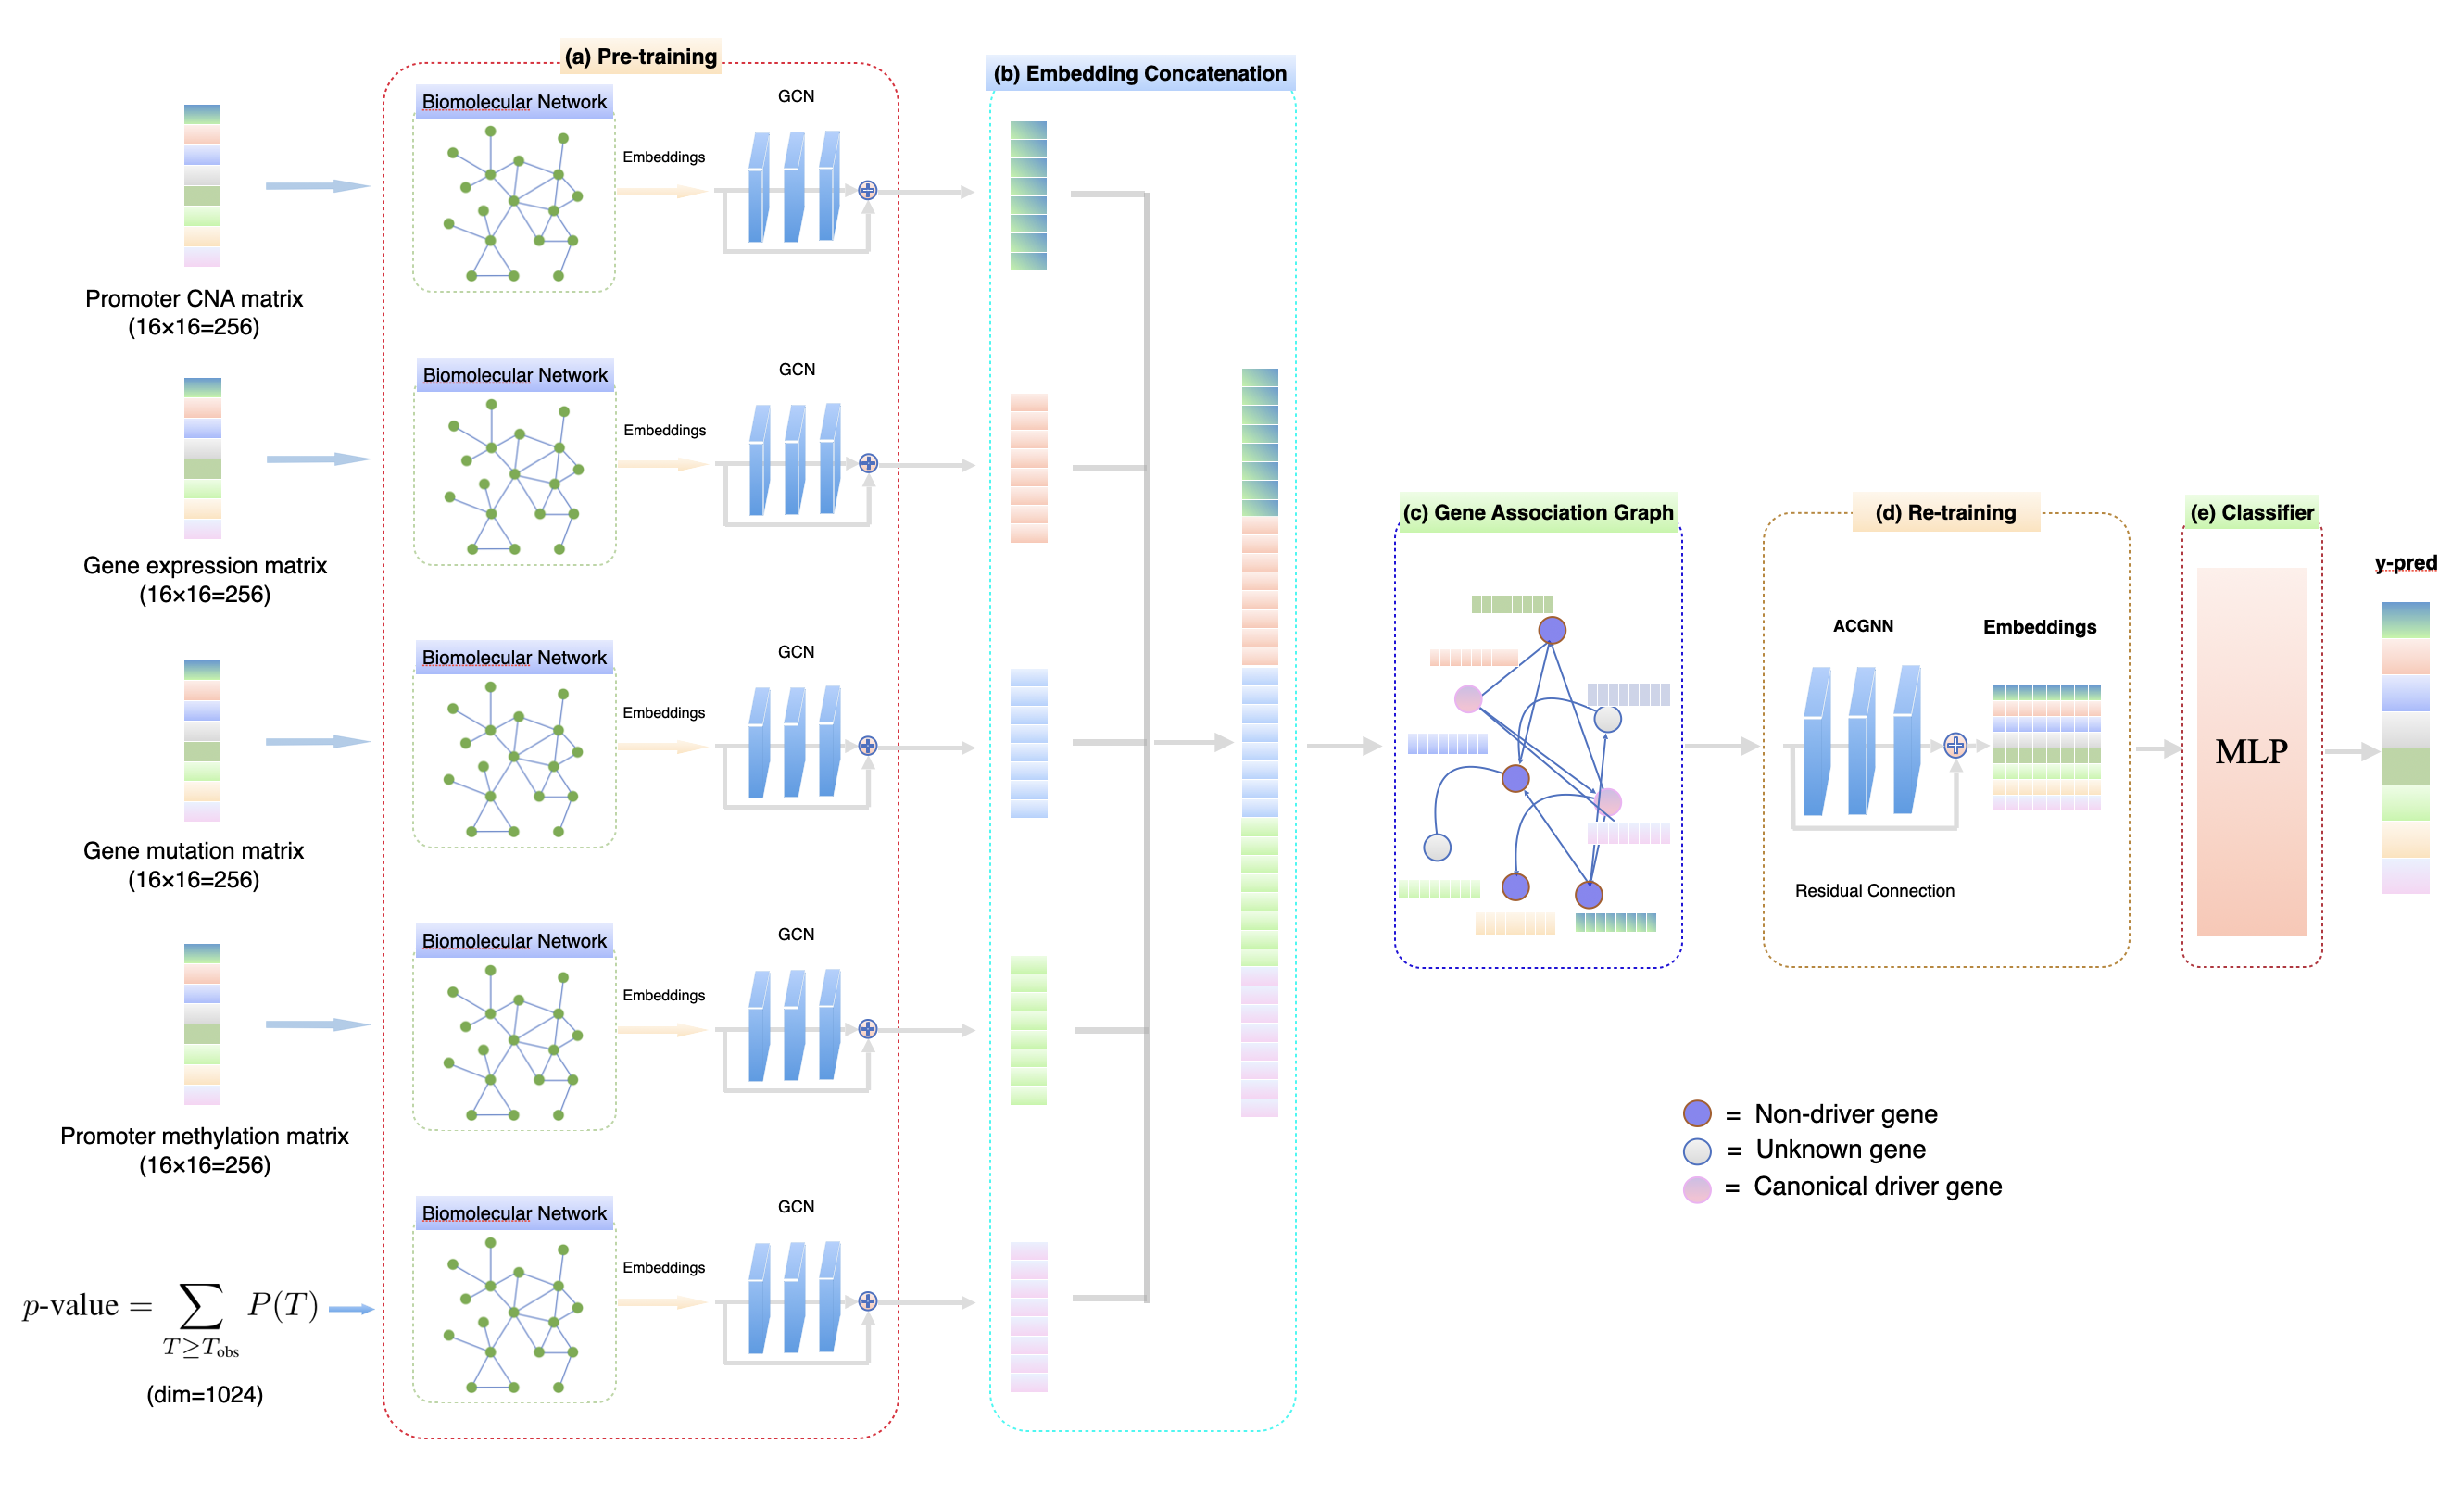
\includegraphics[width=18cm]{images/__overview_framework.png}
	%%\includegraphics[width=9.5cm]{images/_test_f1_vs_latent_dim_hid16_head4_lay8_epo1_5i298.png}
	\vspace{0.5cm} % Adjust the space as needed   
	\caption{Overview of the ACGNN framework.
		(a) Multi-omics biomolecular networks are constructed for gene expression, mutation, and promoter DNA methylation data. Embeddings are extracted using GCN, and PPI network embeddings are integrated through Fisher's exact test.
		(b) Multi-omics embeddings are concatenated to form unified feature representations, combining topological, statistical, and multi-omics data.
		(c) A gene embedding graph is created, where nodes represent genes, and edges capture relationships between concatenated embeddings.
		(d) The ACGNN model refines node embeddings using an adaptive mechanism that dynamically tunes the polynomial order and residual connections, producing low-dimensional representations.
		(e) A binary classifier predicts driver and non-driver genes, outputting probabilities for each gene.}
	\label{overview}
\end{figure*}

\subsection{Data Collection and Preprocessing}

In this study, we utilized the same PPI networks and multi-omics data as EMOGI and HGDC to evaluate our method's performance in identifying cancer driver genes. For completeness, we provide a brief overview of these datasets. 
The CPDB \cite{kamburov2011consensuspathdb} is a specialized database that integrates protein-protein interaction (PPI) data with cancer-specific annotations \cite{cpdb_citation}. It sources data from multiple experimental studies, such as The Cancer Genome Atlas (TCGA) \cite{tcga_citation}.
STRING combines data from high-throughput experiments and curated interaction databases \cite{string_citation}. This resource includes experimental data from sources like the Human Protein Atlas \cite{human_protein_atlas_citation}, KEGG \cite{kegg_citation}, Reactome pathways \cite{reactome_citation,wu2010human}, and Gene Ontology \cite{go_citation}.
HIPPIE (Human Integrated Protein-Protein Interaction Environment) focuses on human-specific protein interactions \cite{hippie_citation,alanis2017hippie,huang2018systematic,khurana2013interpretation}. It integrates high-quality experimental data and curated resources like the Molecular Interaction Database (MInt) \cite{mint_citation} and BioGRID \cite{biogrid_citation}.

The PPI Network, obtained from the STRING database \cite{szklarczyk2023string}, limited to high-confidence interactions with scores above 0.85. 
The multi-omics data, sourced from the TCGA database, included gene mutations, DNA methylation, and gene expression profiles. Similar to EMOGI and MNGCL, we focused on cancer types with available data for gene mutations, gene expression, and DNA methylation in both tumor and normal tissues. 

The three computed biological feature indices for genes are the gene mutation rate, the differential DNA methylation rate, and the differential gene expression rate. The gene mutation rate is calculated as the average of single nucleotide variations and copy number aberrations across all samples within a specific cancer type. The differential DNA methylation rate for each gene is calculated by averaging the methylation differences between cancer and normal samples. This averaging is performed across all cases for a given cancer type.
For each gene \(i\) in cancer type \(c\), a measure of dfferential DNA methylation (\(dm_{ci}\)) at its promoter can be defined as the difference in methylation signal between tumor (\(\beta_{ti}\)) and matched normal sample (\(\beta_{ni}\)), averaged across all available samples \(S_c\) for that \(c\):  

\begin{equation}
	dm_{ci} = \frac{1}{|S_c|} \sum_{t \in S_c} (\beta_{ti} - \beta_{ni}),
	\label{eq:dm_ci}
\end{equation}

The differential expression rate of each gene for a specific cancer type is calculated as the log\(_2\) fold change between expression in cancer and matched normal samples, averaged across all samples. The gene expression data, sourced from Wang et al.~\cite{wang2018unifying} was quantile-normalized and batch-corrected using the ComBat method~\cite{johnson2007adjusting}. 


\subsection{Gene Enrichment Analysis}

Gene enrichment analysis was conducted to identify significant associations among genes using Fisher's Exact Test \cite{fisher1992}. The dataset, containing gene interactions, was analyzed to compute p-values for shared interaction partners between gene pairs. False discovery rates (FDR) were controlled using the Benjamini-Hochberg method \cite{benjamini1995controlling}, with adjusted p-values below 0.05 considered significant. Results included gene pairs, shared partners, p-values, and significance labels. 

\subsection{ACGNN}	
	The Adaptive Chebyshev Graph Neural Network (ACGNN) framework integrates four types of multi-omics data: gene expression, gene mutation, promoter DNA methylation, and copy number alterations (CNA). For each data type, a corresponding biomolecular network \( G_i = (V, E) \) is constructed, where \( V \) represents genes and \( E \) represents interactions. Node embeddings for each network are obtained using Chebyshev spectral filtering. The extracted embeddings capture essential molecular interactions within each data type (Figudetire~\ref{overview}(a)).
	
	To incorporate additional topological information, PPI network embeddings are computed using Fisher’s exact test on enrichment analysis based on gene sets, utilizing the p-value as a significance measure. These topological embeddings provide structural insights into gene interactions.
	
	For each type of multi-omics data, 16 cancer-specific datasets are used to compute node embeddings of size 16, leading to a 256-dimensional feature vector per data type:
	\begin{equation}
		\mathbf{H}_i = \text{Concat}(\mathbf{h}_1, \mathbf{h}_2, ..., \mathbf{h}_{16}) \in \mathbb{R}^{256}
	\end{equation}
	where \( \mathbf{h}_j \) represents the embedding from the \( j \)-th dataset. The four vectors from different omics sources are concatenated to form a 1024-dimensional feature representation:
	\begin{equation}
		\mathbf{H}_{\text{multi-omics}} = \text{Concat}(\mathbf{H}_{\text{GE}}, \mathbf{H}_{\text{GM}}, \mathbf{H}_{\text{DM}}, \mathbf{H}_{\text{CNA}}) \in \mathbb{R}^{1024}
	\end{equation}
	
	Finally, the integrated multi-omics representation is concatenated with the PPI network embeddings to incorporate additional structural information:
	\begin{equation}
		\mathbf{H}_{\text{final}} = \text{Concat}(\mathbf{H}_{\text{multi-omics}}, \mathbf{H}_{\text{topological}}) \in \mathbb{R}^{2048}
	\end{equation}
	This final 2048-dimensional embedding serves as the comprehensive node representation, integrating molecular and structural information into the graph model (Figure~\ref{overview}(b)).
	
	Using these embeddings, a gene embedding graph is constructed, where nodes represent genes and edges capture relationships between them (Figure~\ref{overview}(c)). The ChebNet model refines the node representations through residual connections, which preserve the original feature information while enabling deeper feature transformations (Figure~\ref{overview}(d)).
	
	Finally, a binary classifier, implemented as a multi-layer perceptron (MLP) with a sigmoid activation function, predicts driver and non-driver genes (Figure~\ref{overview}(e)). The output is a probability score for each gene, representing its likelihood of being a cancer driver.
	

\begin{algorithm}
	\caption{ACGNN Method}
	\label{alg:acgnn}
	\textbf{Input:} Graph \( G = (V, E) \), node features \( \mathbf{H}^{(0)} \), rescaled Laplacian matrix \( \tilde{L} \), Chebyshev order \( k \), learnable weight matrices \( \Theta_j \), model parameters.\\
	\textbf{Output:} Predicted output \( Y \).
	
	\begin{algorithmic}[1]
		\State \textbf{Initialize:} Node features \( \mathbf{H}^{(0)} \) and Laplacian matrix \( \tilde{L} \).
		\State \( T_0(\tilde{L}) \leftarrow I \), \( T_1(\tilde{L}) \leftarrow \tilde{L} \)
		
		\For{\( j = 2 \) to \( k \)} \Comment{Compute Chebyshev polynomials}
		\State \( T_j(\tilde{L}) \leftarrow 2\tilde{L} T_{j-1}(\tilde{L}) - T_{j-2}(\tilde{L}) \)
		\EndFor
		
		\State \(\mathbf{H}^{(l+1)} \leftarrow \text{ReLU}\left( \sum_{j=0}^{k} \Theta_j T_j(\tilde{L}) \mathbf{H}^{(l)} \right) \)
		
		\State \(\mathbf{H}^{(l+1)} \gets \text{BatchNorm}(\mathbf{H}^{(l+1)})\)
		\State \(\mathbf{H}^{res} \gets \mathbf{H}^{(l+1)}\)  \Comment{Store residual connection}
		\State \(\mathbf{H}^{(l+2)} \gets \text{ReLU}\left( \sum_{j=0}^{k} \Theta_j T_j(\tilde{L}) \mathbf{H}^{(l+1)} \right) \)
		\State \(\mathbf{H}^{(l+2)} \gets \mathbf{H}^{(l+2)} + \mathbf{H}^{res} \) \Comment{Add residual}
		\State \(\mathbf{H}^{(l+2)} \gets \text{Dropout}(\mathbf{H}^{(l+2)})\)
		\State \( Y \gets \text{MLP}(\mathbf{H}^{(l+2)}) \)
		
		\State \Return \( Y \)
	\end{algorithmic}
\end{algorithm}


\subsection{Model Training and Inference}
	We implement ACGNN using PyTorch and DGL. The network architecture consists of two Chebyshev convolution layers followed by a Multi-Layer Perceptron (MLP). First, bidirectional graphs are constructed for biomolecular networks, incorporating pretrained embeddings as node features. Node labels are assigned as follows: 1 for driver genes, 0 for non-driver genes, and -1 for unlabeled genes.
	
	To define the training and testing sets, we apply the following masking strategy: the training mask includes all labeled nodes, while the testing mask allows all nodes to be evaluated. To ensure computational stability, self-loops are added to the graph, enabling nodes with no incoming edges to maintain connectivity. The model's feature dimensions are configured as follows: the input feature dimension is set to 128, the hidden feature dimension to 128, and the output dimension to 1 for binary classification.

	We use focal loss function \cite{lin2018focal}, given by Equation~\ref{eq:focal_loss}, to extend the standard Binary Cross-Entropy (BCE) loss to address class imbalance by reducing the loss contribution from well-classified examples and focusing more on hard-to-classify samples.
\begin{equation}
	\begin{aligned}
		L_{\text{focal}} = & - \alpha \left( 1 - h \right)^\gamma y \log(h) \\
		& - (1 - \alpha) h^\gamma (1 - y) \log(1 - h).
	\end{aligned}
	\label{eq:focal_loss}
\end{equation}

where \( y \) is the ground truth label, \( h \) is the predicted probability after applying the sigmoid activation function, \( \alpha \) is a weighting factor that balances the positive and negative classes, and \( \gamma \) is a focusing parameter that adjusts the impact of easy versus hard examples. A higher value of \( \gamma \) reduces the relative loss contribution from well-classified samples, placing greater emphasis on misclassified ones. The term \( (1 - h)^\gamma \) scales down the loss for correctly classified positive samples, whereas \( h^\gamma \) does the same for negative samples.

	
	By incorporating these terms, focal loss mitigates the dominance of easily classified examples, ensuring that the model prioritizes learning from challenging cases. This is particularly useful in imbalanced datasets where the positive class, such as cancer driver genes, is significantly underrepresented compared to the negative class.
	
	Node features and graph data are passed through the model to compute logits, which are then used to calculate the training loss based on the ground truth labels for nodes identified by the training mask. Predictions are generated for all nodes by applying a sigmoid activation to the computed logits, yielding the probabilities of each node belonging to the positive class. The pseudocode for executing our model is provided in Algorithm~\ref{alg:acgnn}.
	

\setlength{\tabcolsep}{3pt}  % Reduce column spacing
\begin{table}[h!]
	\centering
	\captionsetup{font=small}
	\scriptsize
	\begin{tabular}{@{}l*{6}{>{\centering\arraybackslash}p{1.2cm}}@{}}
		\toprule
		\textbf{Method} & \textbf{Layers} & \textbf{Input} & \textbf{Hidden} & \textbf{Output} & \textbf{Params} \\ 
		\midrule
		ACGNN     & 5 & 2048 & 1024 & 1 & 7,346,177 \\ 
		HGDC      & 3 & 2048  & 1024 & 1 & 4,202,497 \\ 
		EMOGI     & 3 & 2048  & 1024 & 1 & 4,202,497 \\ 
		MTGCN     & 3 & 2048 & 1024 & 1 & 4,198,401 \\
		GCN       & 3 & 2048 & 1024 & 1 & 4,198,401  \\ 
		GAT       & 3 & 2048 & 1024 & 1 & 4,202,497  \\ 
		GraphSAGE & 3 & 2048 & 1024 & 1 & 7,344,129 \\
		GIN       & 3 & 2048  & 1024 & 1 & 6,297,601 \\ 
		Chebnet   & 3 & 2048 & 1024 & 1 & 10,489,857 \\ 
		\bottomrule
	\end{tabular}
	\caption{Details of model architectures across different methods.}
	\label{tab:model_arch}
\end{table}



\begin{table*}[ht]
	\centering
	\scriptsize
	%\captionsetup{font=scriptsize}
	\captionsetup{font=footnotesize}
	%\caption{Comparison of Models in CPU/GPU Usage and Time Cost per Epoch}
	\begin{tabular}{l*{6}{>{\centering\arraybackslash}p{1.8cm}}}
		\toprule
		\textbf{Model} & \multicolumn{2}{c}{\textbf{CPDB}} & \multicolumn{2}{c}{\textbf{STRING}} & \multicolumn{2}{c}{\textbf{HIPPIE}} \\
		\cmidrule(lr){2-3} \cmidrule(lr){4-5} \cmidrule(lr){6-7}
		& \textbf{CPU/GPU Usage} & \textbf{Time/Epoch} & \textbf{CPU/GPU Usage} & \textbf{Time/Epoch} & \textbf{CPU/GPU Usage} & \textbf{Time/Epoch} \\
		\midrule
		ACGNN    & 3.17M/87.51M & 0.0426s & 3.78M/87.04M & 0.0328s & 3.14M/87.51M & 0.0227s\\
		HGDC     & 3.28M/55.75M & 0.0573s & 3.13M/55.29M & 0.0227s & 3.73M/55.75M & 0.0358s \\
		EMOGI   & 3.23M/55.75M & 0.0573s & 3.08M/55.29M & 0.0348s & 3.61M/55.75M & 0.0227s \\
		MTGCN   & 3.22M/55.72M & 0.0497s & 3.12M/55.25M & 0.0301s & 3.25M/55.72M & 0.0490s \\
		GCN     & 3.23M/55.72M & 0.0470s & 3.11M/55.25M & 0.0329s & 3.33M/55.72M & 0.0429s\\
		GAT     & 3.23M/55.75M & 0.0880s & 3.11M/55.29M & 0.1417s & 3.27M/55.75M & 0.0626s\\
		GrpahSAGE     & 3.17M/87.49M & 0.0532s & 3.25M/87.02M & 0.0210s & 3.18M/87.49M & 0.0330s \\
		GIN     & 3.17M/87.50M  & 0.0528s & 3.26M/87.04M & 0.0213s& 3.20M/87.50M & 0.0378s \\
		ChebNet & 3.22M/119.32M & 0.0622s & 3.13M/118.79M & 0.0241s & 3.16M/119.32M & 0.0453s \\
		\bottomrule
	\end{tabular}
	\caption{Comparison of models in CPU/GPU usage and time cost per epoch on the different PPI networks: CPDB, STRING, and HIPPIE.}
	\label{tab:consume_gpu}
\end{table*}


\begin{table}[ht]
	\centering
	\scriptsize
%\captionsetup{font=scriptsize}
\captionsetup{font=footnotesize}
	\begin{tabular}{l*{6}{>{\centering\arraybackslash}p{0.8cm}}}
		\toprule
		\textbf{Method} & \multicolumn{2}{c}{\textbf{CPDB}} & \multicolumn{2}{c}{\textbf{STRING}} & \multicolumn{2}{c}{\textbf{HIPPIE}} \\
		\cmidrule(lr){2-3} \cmidrule(lr){4-5} \cmidrule(lr){6-7}
		& \textbf{AUROC} & \textbf{AUPRC} & \textbf{AUROC} & \textbf{AUPRC} & \textbf{AUROC} & \textbf{AUPRC} \\
		\midrule
		ACGNN & 0.9652 & 0.9783 & 0.9578 & 0.9738 & 0.9297 & 0.9597 \\
		HGDC & 0.6776 & 0.7288 & 0.7133 & 0.7740 & 0.6525 & 0.7634 \\
		EMOGI & 0.6735 & 0.7230 & 0.81846 & 0.8737 & 0.6672 & 0.7960 \\
		MTGCN & 0.6862 & 0.7712 & 0.7130 & 0.7878 & 0.6762 & 0.7785 \\
		GCN & 0.6915 & 0.7730 & 0.6688 & 0.7681 & 0.6708 & 0.7675 \\
		GAT & 0.6670 & 0.7086 & 0.8166 & 0.8791 & 0.6478 & 0.7496 \\
		GraphSAGE & 0.6664 & 0.7522 & 0.6166 & 0.7182 & 0.6571 & 0.7624 \\
		GIN & 0.5836 & 0.6405 & 0.5173& 0.5918 & 0.5844 & 0.6791 \\
		Chebnet & 0.8017 & 0.8622 & 0.8777 & 0.9159 & 0.7409 & 0.8443 \\
		\bottomrule
	\end{tabular}
	\caption{Performance comparison of different methods across three biological networks: CPDB (pathway-based network), STRING (protein-protein interaction network), and HIPPIE (high-confidence protein interaction network).}
	\label{tab:roc_pr}
\end{table}

\begin{table}[ht]
	\centering
	\scriptsize
%\captionsetup{font=scriptsize}
\captionsetup{font=footnotesize}
	\begin{tabular}{l*{6}{>{\centering\arraybackslash}p{0.8cm}}}
		\toprule
		& \multicolumn{2}{c}{\textbf{CPDB}} & \multicolumn{2}{c}{\textbf{STRING}} & \multicolumn{2}{c}{\textbf{HIPPIE}} \\
		\cmidrule(lr){2-3} \cmidrule(lr){4-5} \cmidrule(lr){6-7}
		& \textbf{AUROC} & \textbf{AUPRC} & \textbf{AUROC} & \textbf{AUPRC} & \textbf{AUROC} & \textbf{AUPRC} \\
		\midrule
		ACGNN & 0.9652 & 0.9783 & 0.9578 & 0.9738 & 0.9297 & 0.9597 \\
		AC256x1 & 0.9315& 0.9527 & 0.9054 & 0.9464 & 0.8551 & 0.9129 \\
		AC256x2 & 0.9382& 0.9610 & 0.9413 & 0.9630 & 0.9112 & 0.9378 \\
		AC256x4 & 0.9495& 0.9657 & 0.9489 & 0.9634 & 0.8934 & 0.9388 \\
		AC1024x1 & 0.8481 & 0.9045 & 0.8653 & 0.9182 & 0.9288 & 0.9504 \\
		\bottomrule
	\end{tabular}
	\caption{The ablation experimental results of the different networks.}
	\label{tab:roc_pr_ablate}
\end{table}



%\begin{figure}[H]
%	\centering
%	\includegraphics[width=0.7\textwidth]{images/ggnet_kde.png}
%	\caption{Kernel Density Estimation (KDE) plot illustrating the distribution of interaction degrees for predicted driver genes and other genes. The x-axis represents the inteaction degree, and the y-axis represents the density.}
%	\label{fig:kde_plot}
%\end{figure}	
%\bigskip
%\vspace{0.5cm} 